\documentclass[11pt]{article}

\usepackage{classDM17}
\usepackage{hyperref}
\usepackage{listings}

\title{Assignment 6: Graphs}
\author{Christohper Mertin/\verb~u1010077~\\
        \url{cmertin@cs.utah.edu}}
\date{\today}


\begin{document}
\maketitle

%\end{titlepage}




%%%%%%%%%%%%%%%%%%%%%%%%%%%%%%%%%%%%%%%%%%%%%%%%%%%%
%%%%%%%%%%%%%%%%%%%%%%%%%%%%%%%%%%%%%%%%%%%%%%%%%%%%
%%%%%%%%%%%%%%%%%%%%%%%%%%%%%%%%%%%%%%%%%%%%%%%%%%%%
\section*{Overview}

In this assignment you will explore different approaches to analyzing Markov chains.  

You will use one data sets for this assignment:
\begin{itemize} \denselist
\item \href{http://www.cs.utah.edu/~jeffp/teaching/cs5140/A6/M.dat}{\texttt{http://www.cs.utah.edu/\~{}jeffp/teaching/cs5140/A6/M.dat}}
%\item \href{http://www.cs.utah.edu/~jeffp/teaching/cs5140/A6/L.dat}{\texttt{http://www.cs.utah.edu/\~{}jeffp/teaching/cs5140/A6/L.dat}}
\end{itemize}
These data sets are in matrix format and can be loaded into MATLAB or OCTAVE.  By calling 
\\
\texttt{load filename} (for instance \texttt{load M.dat})
\\
it will put in memory the the data in the file, for instance in the above example the matrix \texttt{M}.  You can then display this matrix by typing 
\texttt{M}

\vspace{.1in}

\emph{As usual, it is highly recommended that you use LaTeX for this assignment.  If you do not, you may lose points if your assignment is difficult to read or hard to follow.  Find a sample form in this directory:
\url{http://www.cs.utah.edu/~jeffp/teaching/latex/}}


%%%%%%%%%%%%%%%%%%%%%%%%%%%%%%%%%%%%%%%%%%%%%%%%%%%%
%%%%%%%%%%%%%%%%%%%%%%%%%%%%%%%%%%%%%%%%%%%%%%%%%%%%
%%%%%%%%%%%%%%%%%%%%%%%%%%%%%%%%%%%%%%%%%%%%%%%%%%%%
\section{Finding $q_*$ (50 points)}

We will consider four ways to find $q_* = M^t q_0$ as $t \to \infty$.  

\begin{itemize} \denselist
\item[\textsf{Matrix Power:}] 
Choose some large enough value $t$, and create $M^t$.  Then apply $q_* = (M^t) q_0$.  
There are two ways to create $M^t$, first we can just let $M^{i+1} = M^i * M$, repeating this process $t-1$ times.  Alternatively, (for simplicity assume $t$ is a power of $2$), then in $\log_2 t$ steps create $M^{2i}  = M^i * M^i$.  
\item[\textsf{State Propagation:}]
Iterate $q_{i+1} = M * q_i$ for some large enough number $t$ iterations.  
\item[\textsf{Random Walk:}]
Starting with a fixed state $q_0 = [0, 0, \ldots, 1, \ldots, 0, 0]^T$ where there is only a $1$ at the $i$th entry, and then transition to a new state with only a $1$ in the $j$th entry by choosing a new location proportional to the values in the $i$th column of $M$.  
Iterate this some large number $t_0$ of steps to get state $q_0'$.  (This is the \emph{burn in period}.)

Now make $t$ new step starting at $q_0'$ and record the location after each step.  Keep track of how many times you have recorded each location and estimate $q_*$ as the normalized version (recall $\|q_*\|_1 = 1$) of the vector of these counts.  
\item[\textsf{Eigen-Analysis:}]
Compute \texttt{eig(M)} and take the first eigenvector after it has been normalized.  
\end{itemize}

\paragraph{A (20 points):}
Run each method (with $t = 1024$, $q_0 = [1$, $0$, $0$, $\ldots$, $0]^T$ and $t_0 = 100$ when needed) and report the answers.  

\begin{lstlisting}[breaklines]
  Matrix Power
============
[[ 0.03575751]
 [ 0.05721201]
 [ 0.0580922 ]
 [ 0.07921664]
 [ 0.08581802]
 [ 0.06601386]
 [ 0.15790516]
 [ 0.17163604]
 [ 0.13730883]
 [ 0.15103972]]

State Propogation
=================
[[ 0.03575751]
 [ 0.05721201]
 [ 0.0580922 ]
 [ 0.07921664]
 [ 0.08581802]
 [ 0.06601386]
 [ 0.15790516]
 [ 0.17163604]
 [ 0.13730883]
 [ 0.15103972]]

Random Walk
===========
[[ 0.14746094]
 [ 0.10742188]
 [ 0.11328125]
 [ 0.12207031]
 [ 0.13867188]
 [ 0.06640625]
 [ 0.10449219]
 [ 0.05664062]
 [ 0.09570312]
 [ 0.04785156]]

Eigenvalues
===========
[[ 0.10238015]
 [ 0.16380824]
 [ 0.16632836]
 [ 0.2268114 ]
 [ 0.24571235]
 [ 0.1890095 ]
 [ 0.45211073]
 [ 0.49142471]
 [ 0.39313977]
 [ 0.43245374]]
\end{lstlisting}


\paragraph{B (10 points):}
Rerun the \textsf{Matrix Power} and \textsf{State Propagation} techniques with $q_0 = [0.1, 0.1, \ldots, 0.1]^T$.  For what value of $t$ is required to get as close to the true answer as the older initial state?

The decay is quite rapid, and if you take the value using these methods and compute the normed difference between the true value and this method, as the following

\begin{align*}
  \frac{\left|\left| q_{\star} - q_{\star}^{\prime}\right|\right|}{\left|\left| q_{\star}\right|\right|}
\end{align*}

Then we can get an idea on the ``percentage'' that it is off. If we look at the figure below, we see that around $t\approx 50$ gives essentially the same value.

\begin{figure}[h]
\centering
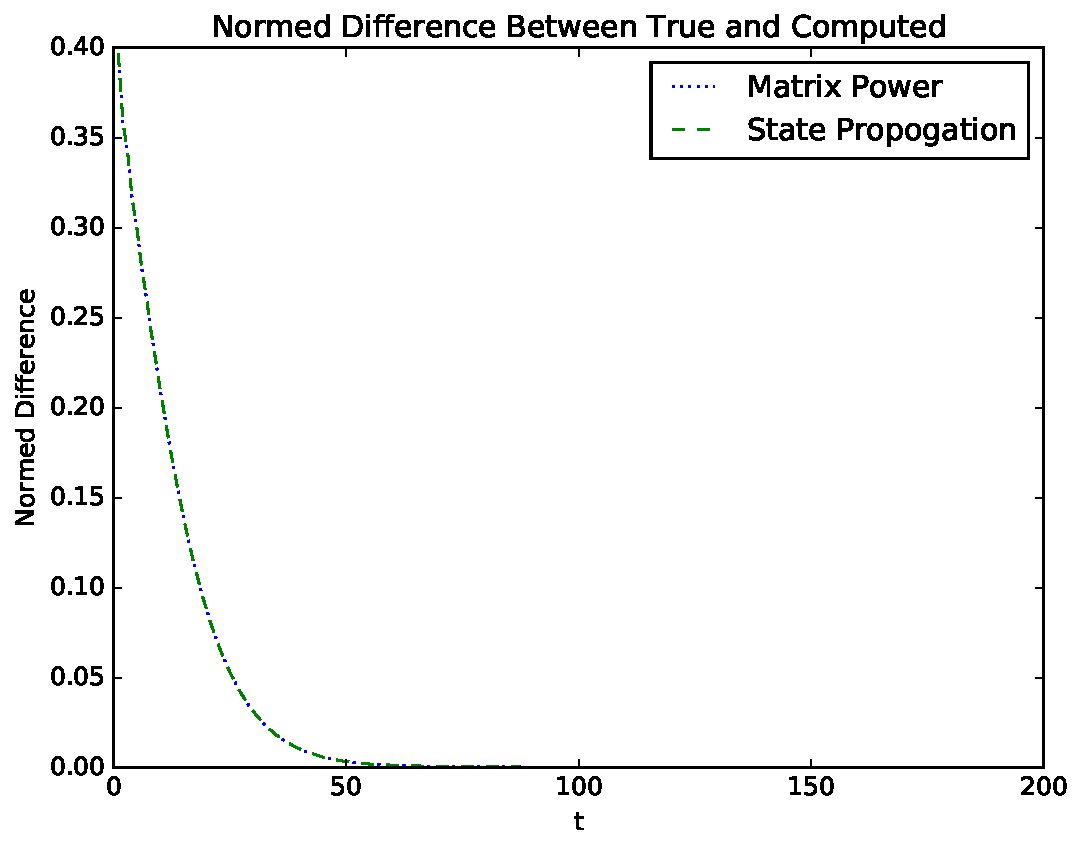
\includegraphics[width=.75\linewidth]{partb.pdf}
\end{figure}

After 200 iterations we have the same values, which can be seen below.

\begin{lstlisting}[breaklines]
Matrix Power
============
[ 0.03575751  0.05721201  0.0580922   0.07921664  0.08581802  0.06601386
  0.15790516  0.17163604  0.13730883  0.15103972]

State Propogation
=================
[ 0.03575751  0.05721201  0.0580922   0.07921664  0.08581802  0.06601386
  0.15790516  0.17163604  0.13730883  0.15103972]
\end{lstlisting}

\paragraph{C (12 points):}
Explain at least one \textbf{Pro} and one \textbf{Con} of each approach.  
The \textbf{Pro} should explain a situation when it is the best option to use.  
The \textbf{Con} should explain why another approach may be better for some situation.  

\begin{itemize}
  \item Matrix Power

    Pro: Accurate Equilibrium Estimation

    Con: Computationally Expensive $\mathcal{O}(\log(t))$

  \item State Propogation

    Pro: Similar to matrix power, easy to implement

    Con: Computationally Expensive

  \item Random Walk

    Pro: Scalable and allows for less complexity $\mathcal{O}(\left|\text{nodes}\right|\times \left|\text{edges}\right|)$ which allows for analysis over larger graphs

    Con: If the number of iterations are too small the resulting state vector has a wide variance. Another is that Random Walk is subject to the structure of a graph and poorly linked clusters might cause it to become stuck.

    \item Eigen Analysis
      
      Pro: Keeps the structure

      Con: Computationally Expensive
\end{itemize}

\paragraph{D (4 points):}
Is the Markov chain \emph{ergodic}?  Explain why or why not.  

A Markov chain is ergodic if there exists a stationary state, thereby preventing the three conditions discussed in class and allowing one to go from any state to any other state. A stationary state can be seen as $x$ such that $x = x^{T}M$. This is the case for $M$ it is true that $[0.1,\ldots,0.1]^{T} = [0.1,\ldots,0.1]^{T}M$. Therefore, the matrix is ergodic.

\paragraph{E (4 points):}
Each matrix row and column represents a node of the graph, label these from $1$ to $10$ starting from the top and from the left.  
What nodes can be reached from node $4$ in one step, and with what probabilities?  



\end{document}
